The primary objective of this thesis is to implement and assess the potentials and limitations of integrating LLM-based automated bug fixing into \ac{CI}. We aim to answer the following research questions to evaluate the feasibility, capabilities and impact on the software development process of this approach.

\begin{itemize}
    \item \textbf{RQ1:} How can LLM-based automated bug fixing be effectively and efficiently integrated into a CI pipeline?
    \item \textbf{RQ2:} What are the potentials and limitations of this integrated approach with respect to repair success rate, execution times and cost-effectiveness?
\end{itemize}

To answer these questions, we structured the process into three phases: preparation, implementation/usage, and evaluation. The process is visualized below in Figure \ref{fig:method-overview}.

\begin{figure}[H]
    \centering
    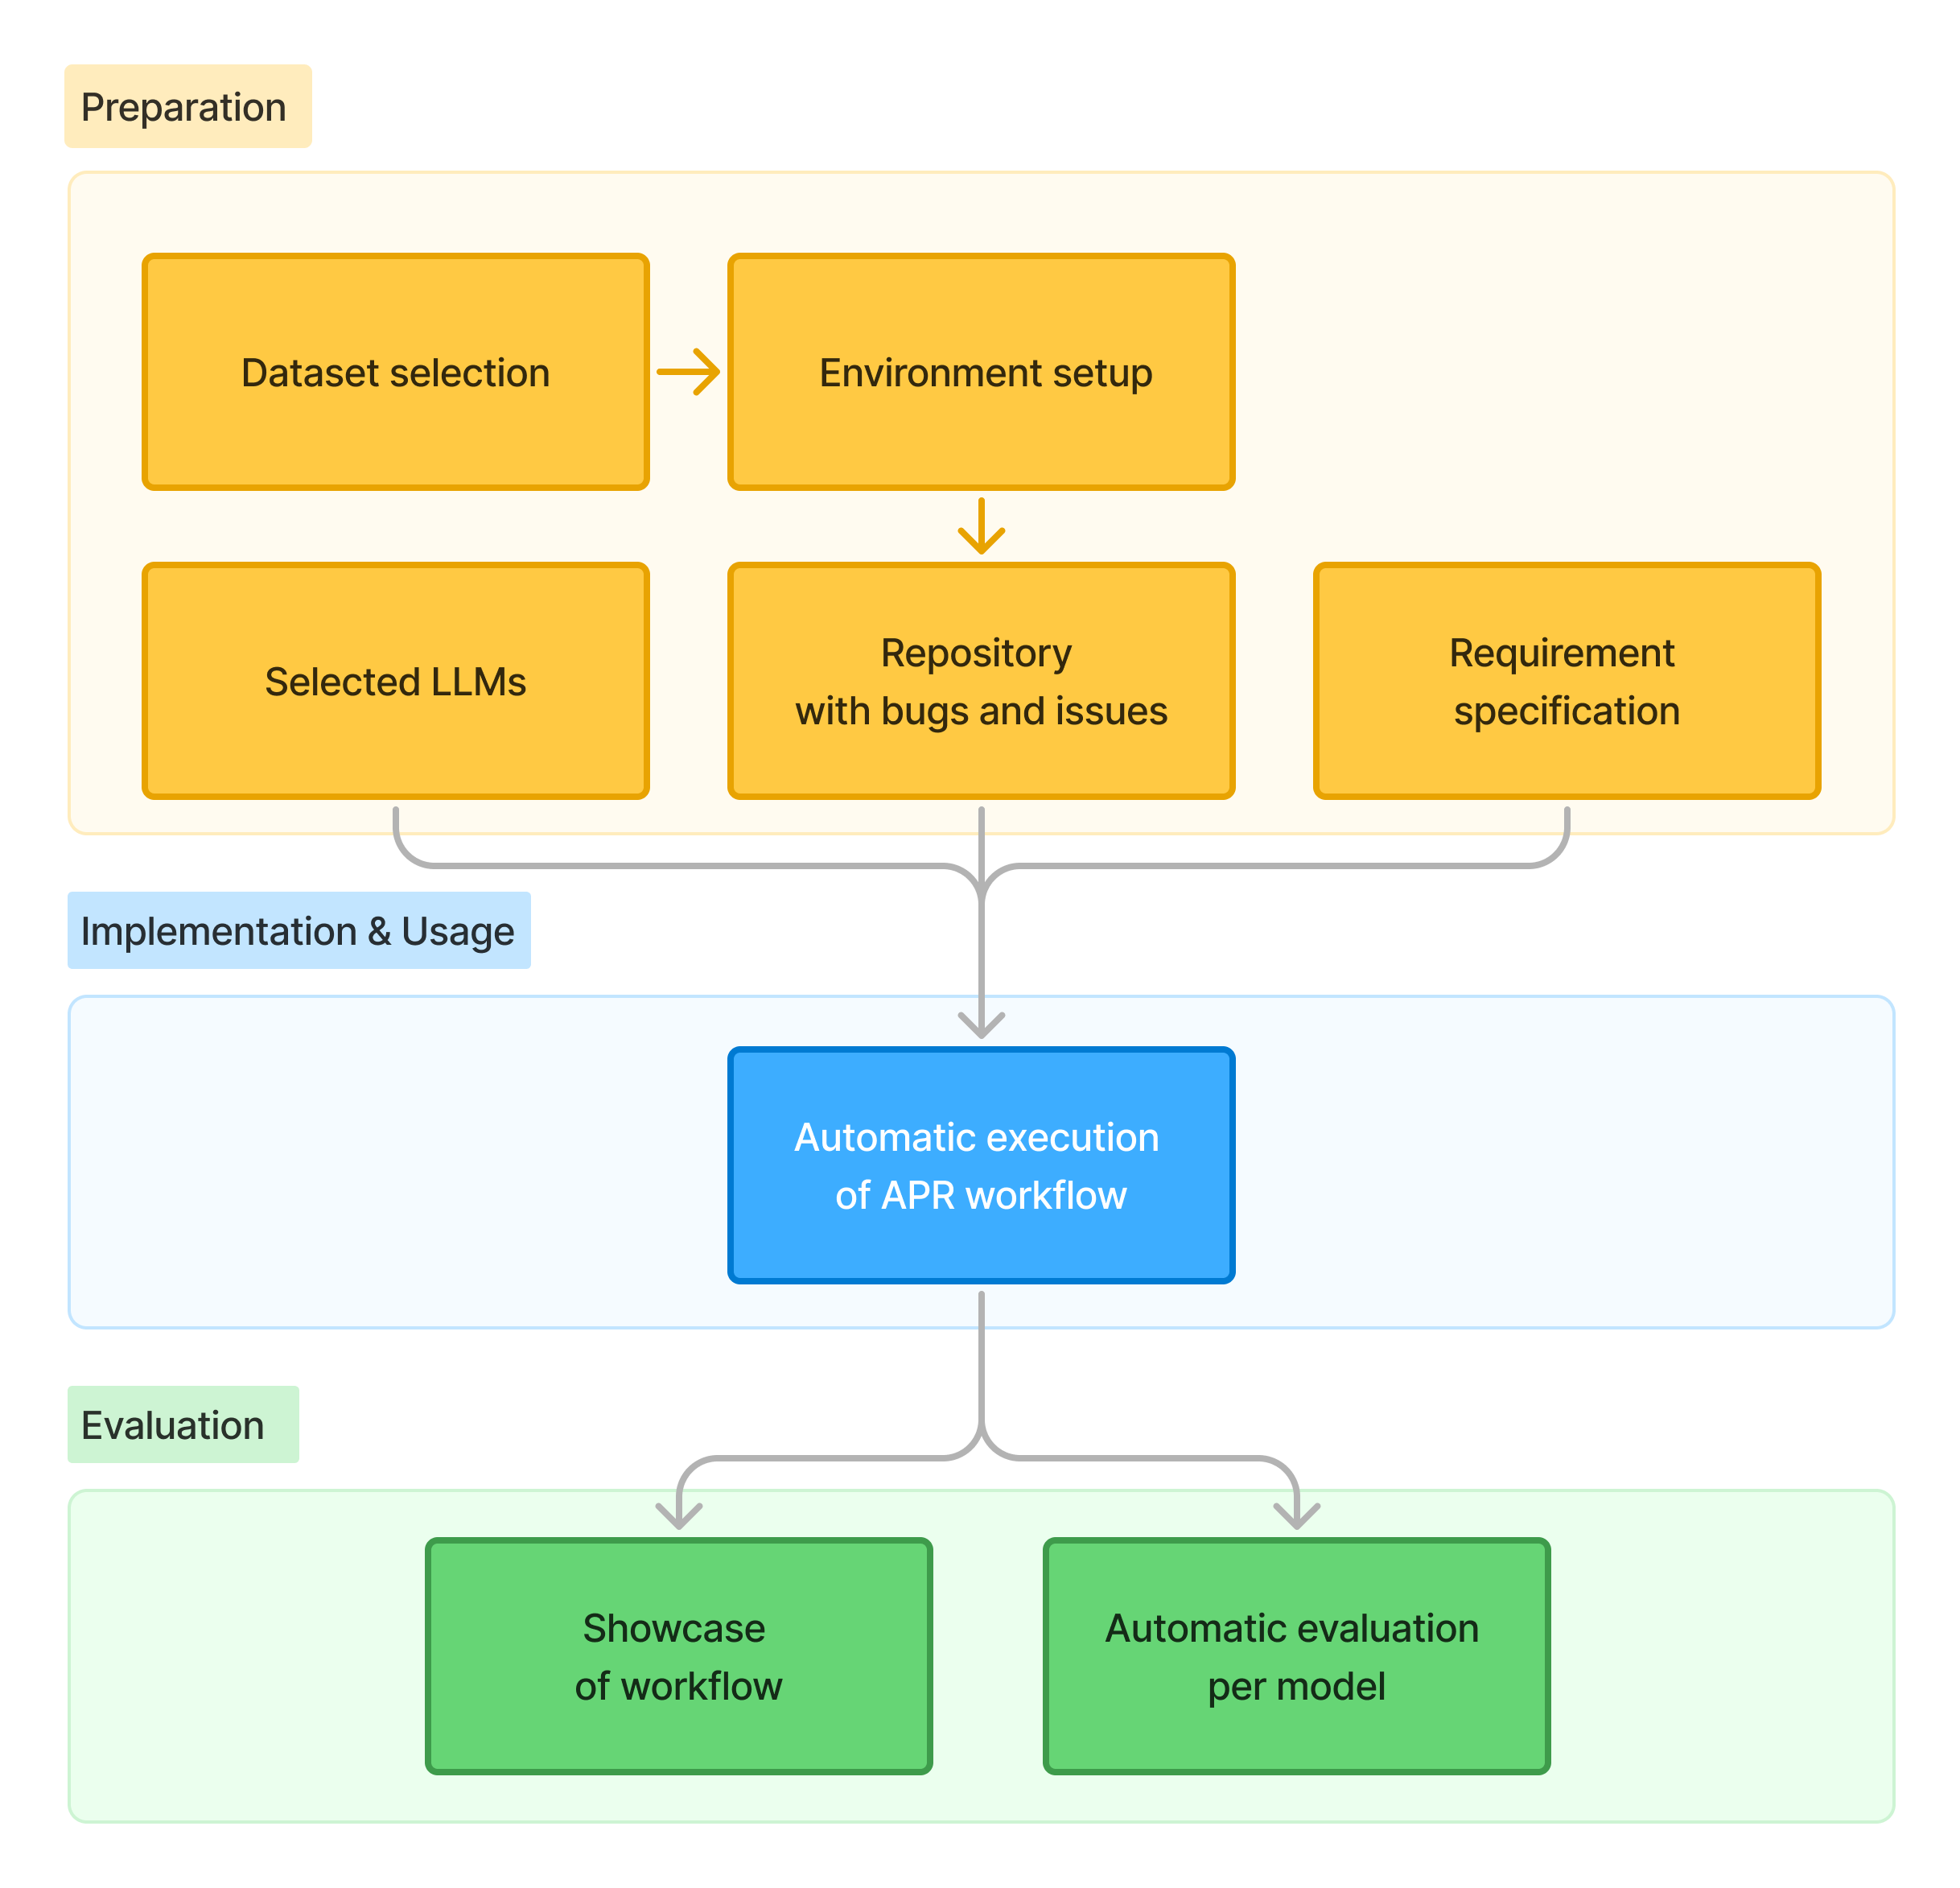
\includegraphics[width=0.95\textwidth]{images/flowcharts/method.png}
    \caption{Thesis methodology approach, Source: own representation}
    \label{fig:method-overview}
\end{figure}

In the preparation phase, we select a suitable \ac{APR} benchmark and a pool of \acp{LLM}. With the benchmark, we set up a realistic development environment on GitHub. By specifying requirements, we lay the groundwork for the implementation of the APR system.
In the second part, we implement the \ac{APR} system based on the requirements.
With this implementation we evaluate the self-developed prototype using the evaluation metrics (listed in Section \ref{section:evaluation}) collected during and after the execution of the APR system. Furthermore, we showcase the resulting workflow of using the system in the prepared repository.
The following sections will go into detail about each of these phases.

\section{Preparation}

For implementing and evaluating our system, we prepared an environment where the system can be integrated, used, and evaluated. This includes selecting a suitable dataset and \acp{LLM}, setting up the environment, and specifying the requirements for the system.

\subsection{Dataset Selection}

For evaluating the effectiveness of our APR integration, we selected the QuixBugs benchmark \cite{linQuixBugsMultilingualProgram2017}. This dataset is well-suited for our purposes due to its focus on small-scale bugs in Python\footnote{QuixBugs also includes translated Java versions, which are excluded from our evaluation.}. It consists of 40 individual files, each containing an algorithmic bug caused by a single erroneous line. Corresponding tests and a corrected version for every file are also included in the benchmark, which allows for seamless repair validation. QuixBugs was developed as a set of challenging problems for developers \cite{linQuixBugsMultilingualProgram2017}, enabling us to evaluate whether our system can take over the cognitively demanding task of fixing small bugs without developer intervention.
Compared to other APR benchmarks \ref{table:benchmarks} like SWE-Bench \cite{jimenezSWEbenchCanLanguage2024}, QuixBugs is relatively small, which allows for accelerated setup and development.

\subsection{Large Language Model Selection} \label{subsection:llm-selection}
For the evaluation of our APR system, we test a selected pool of \acp{LLM}. We evaluate with the latest models\footnote{released before 11 July 2025} from the three vendors that currently dominate AI-assisted coding workflows: Google, OpenAI, and Anthropic. %TODO cite
The models are selected to cover a range of capabilities and costs, with a focus on lower-tier models, allowing us to evaluate the performance, execution times and cost-effectiveness of the APR system. Table \ref{table:llms} shows twelve selected models that are used for evaluation with the following data:
\begin{itemize}
    \item (1) Model Name: The name of the \ac{LLM}.
    \item (1a) Abbreviation: Short identifier used for results and tables.
    \item (2) Context Window Size in Tokens: The maximum number of tokens the model can process in a single request.
    \item (3) Cost per 1M Tokens: The cost of processing 1 million tokens, divided into input and output cost.
    \item (4) Provider Description: Description of the model's characteristics.
    \item (5) Source: The source where the model information was obtained.
\end{itemize}

\begin{longtable}{@{\extracolsep{\fill}} p{3cm} | p{1.3cm} | p{1cm} | p{2.5cm} | p{4cm} | p{1cm} @{}}
    \caption{Characteristics of selected LLMs (21.07.2025)} \label{table:llms}                                                                                                                                                            \\

    \hline
    \textbf{(1)}                      & \textbf{(1a)} & \textbf{(2)} & \textbf{(3)}                           & \textbf{(4)}                                                                                  & \textbf{(5)}              \\
    \hline
    \endfirsthead

    \hline
    \endfoot
    \textbf{gemini-2.0-flash-lite}    & G2F-L         & 1M           & input: \$0.075 \newline output: \$0.30 & Cost efficiency and low latency                                                               & \cite{GeminiModelsGemini} \\ \hline
    \textbf{gemini-2.0-flash}         & G2F           & 1M           & input: \$0.15 \newline output: \$0.60  & Next generation features, speed, and realtime streaming                                       & \cite{GeminiModelsGemini} \\ \hline
    \textbf{gemini-2.5-flash-lite} & G25F-L        & 1M           & input: \$0.10 \newline output: \$0.40  & Most cost-efficient \newline model supporting high throughput                                 & \cite{GeminiModelsGemini} \\ \hline
    \textbf{gemini-2.5-flash}         & G25F          & 1M           & input: \$0.30 \newline output: \$2.50  & Adaptive thinking, cost efficiency                                                            & \cite{GeminiModelsGemini} \\ \hline
    \textbf{gemini-2.5-pro}           & G25P          & 1M           & input: \$1.25 \newline output: \$10.00 & Enhanced thinking \newline and reasoning, multimodal understanding, advanced coding, and more & \cite{GeminiModelsGemini} \\ \hline
    \textbf{gpt-4.1-nano}             & GPT4N         & 1M           & input: \$0.10 \newline output: \$0.40  & Fastest, most cost-effective                                                                  & \cite{ModelsOpenAIAPI}    \\ \hline
    \textbf{gpt-4.1-mini}             & GPT4M         & 1M           & input: \$0.40 \newline output: \$1.60  & Balanced for \newline intelligence, speed, and cost                                           & \cite{ModelsOpenAIAPI}    \\ \hline
    \textbf{gpt-4.1}                  & GPT4          & 1M           & input: \$2.00 \newline output: \$8.00  & Flagship GPT model for complex tasks                                                          & \cite{ModelsOpenAIAPI}    \\ \hline
    \textbf{o4-mini}                  & O4M           & 200k         & input: \$1.10 \newline output: \$4.40  & Optimized for fast, effective reasoning with exceptionally efficient performance in coding    & \cite{ModelsOpenAIAPI}    \\ \hline
    \textbf{claude-3-5-haiku}         & C35H          & 200k         & input: \$0.80 \newline output: \$4.00  & Our fastest model                                                                             & \cite{ModelsOverview}     \\ \hline
    \textbf{claude-3-7-sonnet}        & C37S          & 200k         & input: \$3.00 \newline output: \$15.00 & High-performance model with early \newline extended thinking                                  & \cite{ModelsOverview}     \\ \hline
    \textbf{claude-sonnet-4-0}        & CS40          & 200k         & input: \$3.00 \newline output: \$15.00 & High-performance model                                                                        & \cite{ModelsOverview}     \\
    \hline
\end{longtable}

The exact snapshot versions of each model used are listed in the Appendix \ref{chapter:appendix}.


\subsection{Environment Setup} \label{subsection:environment-setup}
To mirror a realistic software development environment, we prepared a GitHub repository containing the QuixBugs Python dataset. This repository serves as the basis for the bug-fixing process, allowing the system to interact with the codebase and perform repairs.

Using the 40 buggy files, we generate a GitHub issue for each. A consistent issue template is used, capturing only the title of the problem with a minimal description. The generated issues serve as the entry point and communication medium for the APR system. Figure \ref{fig:gh-issue} shows an example of a generated GitHub issue.

\begin{figure}[H]
    \centering
    \includegraphics[width=1\textwidth]{images/github/github_issue.png}
    \caption{Example of a generated GitHub Issue, Source: own representation}
    \label{fig:gh-issue2}
\end{figure}

\subsection{Requirements Specification}

Before the implementation phase, we constructed requirements for the \ac{APR} prototype. We followed the INVEST model, a widely adopted method in Agile software development for engineering requirements \cite{10.5555/984017}. According to the INVEST principles, each requirement was formulated to be independent, negotiable, valuable, estimable, small, and testable. Using this framework, we defined both functional and non-functional requirements. The requirements are precisely defined, verifiable, and easily adaptable to iterative development. Chapter \ref{chapter:requirements} showcases the resulting requirements.

\section{System Implementation}

In this section, we provide a high-level overview of the implemented automated bug fixing \ac{CI} pipeline. Chapter \ref{chapter:implementation} provides a more detailed description of the implementation.

The prototype was developed using iterative prototyping and testing, with a focus on simplicity and extensibility. It is based on the self-developed requirements. An overview of the system is visualized in Figure \ref{fig:high-level} and Figure \ref{fig:apr-core-overview}.

Figure \ref{fig:high-level} shows that once the system is in place, a \ac{CI} pipeline can be triggered by different events. This executes the CI pipeline on a GitHub Action runner. The first pipeline job fetches and filters relevant issues. Resulting issues are passed to the APR Core, which contains the main bug-fixing logic. The APR Core (visualized in Figure \ref{fig:apr-core-overview}) runs in a container and communicates with the configured \acp{LLM} via API to localize and fix the issue. With the generated file edits, the changes are validated and tested. When validation passes, the changes are applied and a pull request is opened on the repository, linking the issue. In case of an unsuccessful repair or exhaustion of the maximum number of attempts, a failure is reported to the issue.

\begin{figure}[H]
    \centering
    \includegraphics[width=1\textwidth]{images/flowcharts/overview.png}
    \caption{Overview of the CI Pipeline, Source: own representation}
    \label{fig:high-level}
\end{figure}

\begin{figure}[H]
    \centering
    \includegraphics[width=1\textwidth]{images/flowcharts/apr_core_overview.png}
    \caption{Overview of the APR Core, Source: own representation}
    \label{fig:apr-core-overview}
\end{figure}



\section{Evaluation} \label{section:evaluation}
%TODO should I mention showcase of results here?
This section describes how we measure the effectiveness, performance and cost of the APR system when integrated into a GitHub repository. We use GitHub Actions' \ac{CI} capabilities in combination with the prepared QuixBugs repository as a base. All twelve selected LLM models from Table \ref{subsection:llm-selection} are evaluated using the prototype. The evaluation is based on data collected during and after a execution of the APR system.

We focus on several key data metrics to assess the system's performance and capabilities in repairing software bugs. These metrics provide insights into effectiveness, performance, reliability, cost and overall impact on the \ac{SDLC}.

Effectiveness of the \acp{LLM} and the approach, is measured by the repair success rate. A repair is considered successful if it passes both the validation stage and the complete test suite provided by QuixBugs. Specifically, an issue is deemed fixed when the generated code is syntactically correct and all associated tests pass without errors.

To assess performance, we analyze collect timings of issue repair attempts. Feasibility is evaluated by estimating the cost of a repair attempt based on the number of tokens and token pricing listed by API providers. GitHub Action minutes are not included in the cost estimation, as 2000 minutes are included in the free tier of GitHub for public repositories \cite{GitHubsPlans}.

Furthermore, we evaluate whether multiple attempts\footnote{equivalent to few shot prompting} can help improve the repair success rate and how this relates to the execution time and cost of the repair process.

Each execution of the APR system collects repair process data. Using self-developed Python scripts, we aggregate the data from different sources for each run. Below, we summarize data collected for each run (Table\ref{table:run-metrics}), each issue processed (Table\ref{table:issue-metrics}), and each stage of an issue repair process (Table \ref{table:stage-metrics}). We use this data to calculate results for  runs testing different configurations with each of the selected \acp{LLM}, which will help in answering RQ2. Table \ref{table:calculations} shows the resulting calculations.

{
\small
\renewcommand{\arraystretch}{1.5}
\begin{longtable}{@{\extracolsep{\fill}} p{3.2cm} | p{7cm} | p{3.5cm} @{}}
    \caption{Summary of metrics collected for each run} \label{table:run-metrics} \\

    \hline
    \textbf{Metric} & \textbf{Description} & \textbf{Source} \\
    \hline
    \endfirsthead

    \hline
    \endfoot
    RunID & Unique identifier for the workflow run & Github Action Runner \\ \hline
    Configuration & Configuration details, including LLM and maximum attempts allowed & Github repository \& \newline APR Core  \\ \hline
    Execution Times & Total time taken for the run & GitHub API \& \newline APR Core \\ \hline
    Job Execution Times & Time taken for each job in the pipeline & Github API \\ \hline
    Issues Processed & Data of issues processed shown in Table \ref{table:issue-metrics} & APR Core \\
    \hline
\end{longtable}
}

{
\small
\renewcommand{\arraystretch}{1.5}
\begin{longtable}{@{\extracolsep{\fill}} p{3.2cm} | p{7cm} | p{3.5cm} @{}}
    \caption{Summary of metrics collected for each processed issue} \label{table:issue-metrics} \\

    \hline
    \textbf{Metric} & \textbf{Description} & \textbf{Source} \\
    \hline
    \endfirsthead

    \hline
    \endfoot
    IssueID & Unique identifier of the issue & Github Issue ID \\ \hline
    Repair Successful & Boolean indicating whether the repair was successful & APR Core \\ \hline
    Number of Attempts & Total attempts made & APR Core \\ \hline
    Execution Time & Time taken to process the issue, including all stages & APR Core \\ \hline
    Tokens Used & Number of tokens processed by the LLM during the repair process & LLM API \\ \hline
    Cost & Cost associated with the repair process, calculated based on tokens * cost per token & APR Core \\ \hline
    Stage Information & Details about each stage of the repair process shown in Table \ref{table:stage-metrics} & APR Core \\
    \hline
\end{longtable}
}

{
\small
\renewcommand{\arraystretch}{1.5}
\begin{longtable}{@{\extracolsep{\fill}} p{3.2cm} | p{7cm} | p{3.5cm} @{}}
    \caption{Summary of metrics collected for each stage} \label{table:stage-metrics} \\

    \hline
    \textbf{Metric} & \textbf{Description} & \textbf{Source} \\
    \hline
    \endfirsthead

    \hline
    \endfoot
    StageID & Unique identifier of the stage & APR Core \\ \hline
    Stage Execution \newline Time & Time taken for stage to complete & APR Core \\ \hline
    Stage Outcome & Outcome of each stage, indicating success, warning or failure & APR Core \\ \hline
    Stage Details & Additional details, such as error or warnings messages & APR Core \\
    \hline
\end{longtable}
}

{
\small
\renewcommand{\arraystretch}{2.5}
\begin{longtable}{@{\extracolsep{\fill}} p{7cm} | >{\centering\arraybackslash}p{7cm} @{}}
    \caption{Run evaluation metrics} \label{table:calculations} \\

    \hline
    \textbf{Metrics} &  \textbf{Calculation} \\
    \hline
    \endfirsthead

    \hline
    \endfoot
    Repair Success Rate & \(\displaystyle\frac{\mathit{Number\ of\ Successful\ Repairs}}{\mathit{Total\ Issues\ Processed}}\) \\ \hline
    Average Execution Time per Issue & \(\displaystyle\frac{\mathit{Total\ Execution\ Time}}{\mathit{Total\ Issues\ Processed}}\) \\ \hline
    Average Cost per Issue & \(\displaystyle\frac{\mathit{Total\ Cost}}{\mathit{Total\ Issues\ Processed}}\) \\ \hline
    APR Core Execution Time & \(\displaystyle\frac{\mathit{Total\ APR\ Core\ Execution\ Time}}{\mathit{Total\ Issues\ Processed}}\) \\ \hline
    CI Pipeline Execution Time & \(\displaystyle\frac{\mathit{Total\ CI\ Pipeline\ Execution\ Time}}{\mathit{Total\ Issues\ Processed}}\) \\ \hline
\end{longtable}
}
